\documentclass[12pt]{article}
\usepackage[english]{babel}
%\usepackage{subcaption}
\usepackage{hyperref}
\usepackage{graphicx}
\usepackage{amsmath}
\graphicspath{{images/}}
\usepackage{geometry}
 \geometry{
 a4paper,
 total={170mm,257mm},
 left=20mm,
 top=20mm,
 }
\begin{document}
\section{Implementation of Lucas-Kanade (LK) template tracker} 
\subsection{Introduction}
In this project we tracked an object or a human being through out the video using Lucas-Kanade (LK) algorithm.

\subsection{Lucas Kanade Algorithm}
The goal of the Lucas-Kanade algorithm is to minimize the sum of squared error between two
images, the template T and the image I warped back onto the coordinate frame of the template.

\begin{figure}[h]
    \centering
    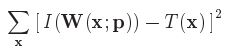
\includegraphics[width=4cm]{error1}
    \caption{Mean Square error}
    \label{fig:Mean Square error}
\end{figure}
Warping I back to compute I (W(x; p)) requires interpolating the image I at the sub-pixel locations W(x; p). The minimization in Equation (3) is performed with respect to p and the sum is
performed over all of the pixels x in the template image T (x). Minimizing the expression in Equation (1) is a non-linear optimization task even if W(x; p) is linear in p because the pixel values
I (x) are, in general, non-linear in x. In fact, the pixel values I (x) are essentially un-related to
the pixel coordinates x. To optimize the expression in Equation (3), the Lucas-Kanade algorithm
assumes that a current estimate of p is known and then iteratively solves for increments to the
parameters $\Delta$p; i.e. the following expression is (approximately) minimized:

\begin{figure}[h]
    \centering
    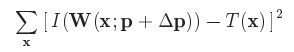
\includegraphics[width=5cm]{error2}
    \caption{Warpped Mean Square error}
    \label{fig:Warpped Mean Square error}
\end{figure}

with respect to $\Delta$p, and then the parameters are update
\begin{equation}
p = p + \Delta p
\end{equation}

These two steps are iterated until the estimates of the parameters p converge. Typically the test for
convergence is whether some norm of the vector $\Delta$p is below a threshold $\varepsilon$; i.e. $||\Delta p|| \leq \varepsilon $ 
\subsection{Pipeline followed}
\begin{enumerate}
\item First step is to crop the template out of the video which we want to track through out the video. The template ($T(x)$) is extracted from the first frame of every video. For this project the following are the templates considered.

\begin{figure}[h]
    \centering
    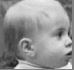
\includegraphics[width=2cm]{babytemplate}
    \caption{Dragon Baby template}
    \label{fig:Dragon Baby template}
\end{figure}

\begin{figure}[h]
    \centering
    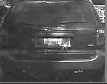
\includegraphics[width=6cm]{cartemplate}
    \caption{Car template}
    \label{fig:Car template}
\end{figure}

\begin{figure}[h]
    \centering
    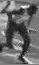
\includegraphics[width=1cm]{bolttemplate}
    \caption{Bolt template}
    \label{fig: Bolt template}
\end{figure}

\item The next step is to perfrom affine transform that warps the current frame so that the template in the first frame is aligned with the warped current frame. The affine transform takes care of the change in scale of the template in the current frame. The obtained image is denoted by $I(W(x;p))$

\item The next step is to compute the error between the warped image and the template.

\begin{figure}[h]
    \centering
    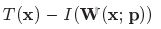
\includegraphics[width=4cm]{error}
    \caption{Error}
    \label{fig: Error}
\end{figure}

\item The next step is computing the gradient $\nabla$I of the warpped image $I(W(x;p))$. Gradient of the image is computed both w.r.t x and y using the Sobel filter.
\begin{equation}
 \nabla I = \left(\frac{\partial I}{\partial x}, \frac{\partial I}{\partial y}\right)
\end{equation}
\item Then the jacobian is computed at (x;p). The jacobian is computed for every point in the warpped image The jacobian is given by :
\begin{equation}
\frac{\partial W}{\partial p} = 
\begin{pmatrix}
x & 0 & y & 0 & 1 & 0 \\
0 & x & 0 & y & 0 & 1
\end{pmatrix}
\end{equation}
\item The next step is to compute the steepest gradient descent. The steepest gradient is given by $\nabla I*\frac{\partial W}{\partial p}$:

\item Then we need to compute the Hessian matrix. The Hessian matrix is given by
\begin{equation}
H = \displaystyle\sum_{x}\left[\nabla I*\frac{\partial W}{\partial p}\right]^T*\left[\nabla I*\frac{\partial W}{\partial p}\right]
\end{equation}

\item Finally computing $\Delta p$ which is the updated parameters of the affine transformation matrix which shift the bounding box of the template to bound the object in the current frame.
\begin{equation}
\Delta p = H^{-1}\displaystyle\sum_{x}\left[\nabla I*\frac{\partial W}{\partial p}\right]^T*\left[T(x) - I(W(x;p))\right]
\end{equation}
 \item We need to iterate this process till $\Delta p$ converges to a small threshold value.
\end{enumerate}
The figure below summarizes the algorithm:
\begin{figure}[h]
    \centering
    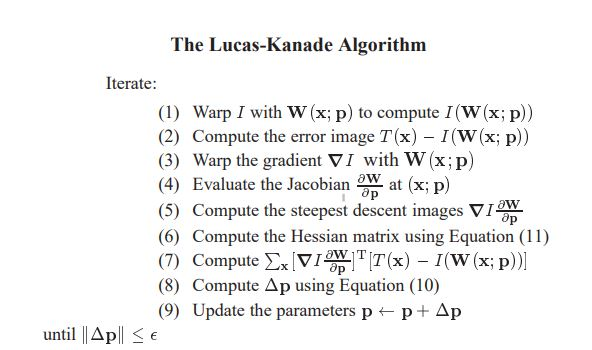
\includegraphics[width=13cm]{lucas}
    \caption{Lucas Kanade Algorithm}
    \label{fig: Lucas Kanade Algorithm}
\end{figure}

\section{Output images by implementing Lucas Kanade}
\subsection{Tracking Bolt}
\begin{figure}[h]
    \centering
    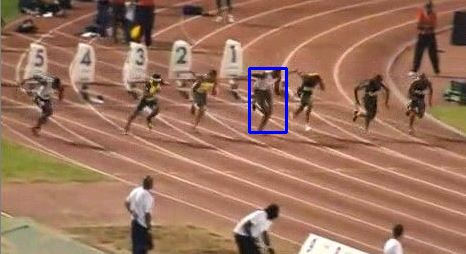
\includegraphics[width=12cm]{trackbolt1}
    \caption{Tracking Bolt}
    \label{fig:Tracking Bolt}
\end{figure}
\newpage
\begin{figure}[h]
    \centering
    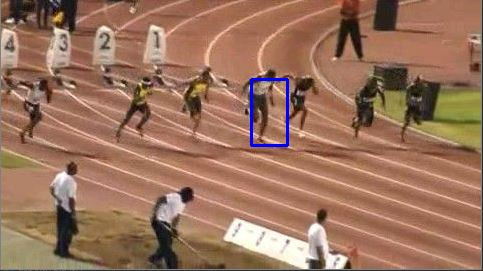
\includegraphics[width=12cm]{trackbolt2}
    \caption{Tracking Car}
    \label{fig:Tracking Car}
\end{figure}

\begin{figure}[h]
    \centering
    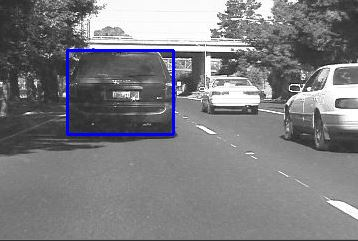
\includegraphics[width=12cm]{trackcar1}
    \caption{Tracking Car}
    \label{fig:Tracking Car}
\end{figure}
\newpage
\begin{figure}[h]
    \centering
    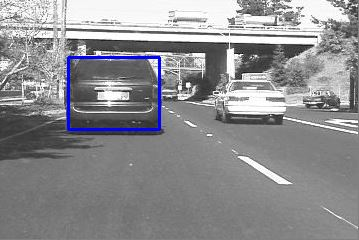
\includegraphics[width=12cm]{trackcar2}
    \caption{Tracking Car}
    \label{fig:Tracking Cat}
\end{figure}

\begin{figure}[h]
    \centering
    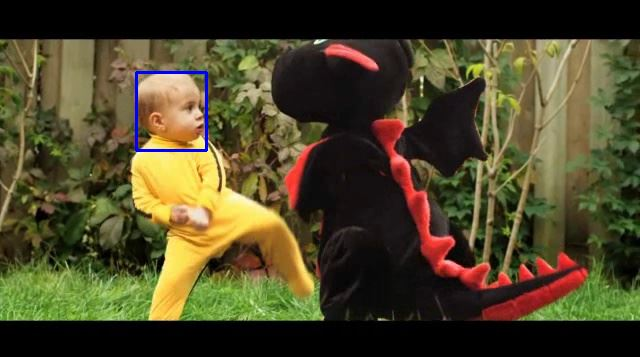
\includegraphics[width=12cm]{trackbaby1}
    \caption{Tracking Baby}
    \label{fig:Tracking Baby}
\end{figure}
\newpage
\begin{figure}[h]
    \centering
    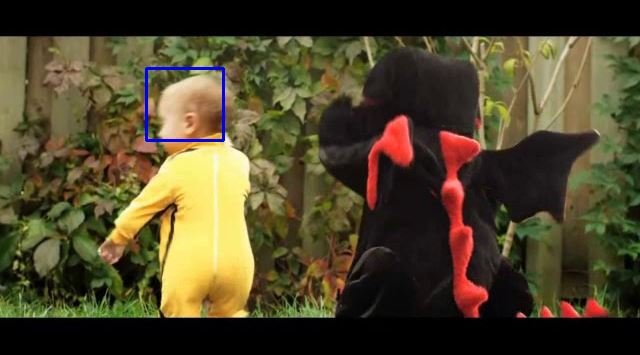
\includegraphics[width=12cm]{trackbaby2}
    \caption{Tracking Baby}
    \label{fig:Tracking Baby}
\end{figure}
\section{Evaluation of the tracker}
Since a taylor approximation is being used, the tracker will work best when 
\begin{enumerate}
  \item Approximation made is close to the template- This means when the object moves really fast in successive frames, the errors induced in the taylor approximation becomes huges and the tracker breaks down.
  \item Brightness of the tracked object remains the same as that of the template 
\end{enumerate}

\textbf{Car tracker} -
The tracker breaks down in the case of car video because the intensity of the frame in the video changes continuously. In the case of the car video, when the car goes into the shadow, the tracker looses the car because the intensity level changes drastically between frames. 
\begin{figure}[h]
    \centering
    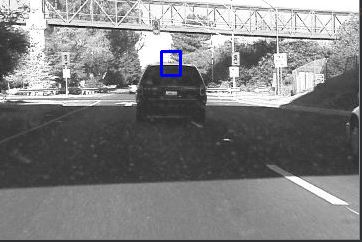
\includegraphics[width=12cm]{trackcar3}
    \caption{Tracking error}
    \label{fig:Tracking error}
\end{figure}

\textbf{Baby tracker}-
The tracker breaks down for the baby as the change is successive frames is slightly big.The baby is just as fast or probably 
faster than usian bolt. \\

\textbf{Usian tracker}-
The tracker breaks for usian bolt as the template used in the first frame(\textbf{usian bolt in a crouched position})is not the same as the template used in successive frames(\textbf{usian bolt in upright}). Template correction-that is, update template with next frame- can be applied but the downside is that if an error is made, it propagates and affects the remaining frames.

In all Usian bolt tracking is the best compared to the others as the shift in successive frames is fairly small and the brightness remains constant.

\section{Robustness to Illumination}
In order to increase the robustness of the tracker, we need to scale the brightness of pixels in each frame so that the average brightness of pixels in the tracked region stays the same as the average brightness of pixels in the template. This can be done by gamma correction.
After increasing the intensity of the frames in the video the following results we re obtained:
\begin{figure}[h]
    \centering
    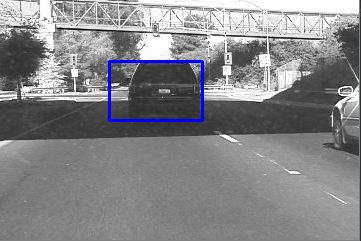
\includegraphics[width=11cm]{trackcar4}
    \caption{Tracking error}
    \label{fig:Tracking error}
\end{figure}

\begin{figure}[h]
    \centering
    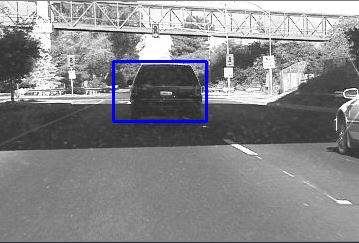
\includegraphics[width=11cm]{trackcar5}
    \caption{Tracking error}
    \label{fig:Tracking error}
\end{figure}

\section{Team Members:}
1. Eashwar Sathyamurthy
2. Akwasi A Obeng
3. Achal P Vyas
\section{Output Videos:}
To access output videos please use this \href{https://drive.google.com/drive/folders/1nbAUx-p-eyOWts9neJgAPA8YATY4ekmI?usp=sharing}{\underline{link}}.

\end{document}
